\section{Implementazione}
In questa sezione verranno descritti gli strumenti utilizzati per implementare i componenti che
permettono alla piattaforma di erogare i propri servizi.
La motivazione principale che ha portato alla scelta delle tecnologie di seguito elencate è il \textit{know-how} aziendale.

\subsection{Linguaggio}
\subsubsection{Typescript}
Typescript\cite{Typescript} è un linguaggio open source sviluppato da Microsoft.

È un \textit{super-set} del linguaggio JavaScript, permettendone l'estensione
con l'introduzione di un meccanismo di tipizzazione statico e il supporto alla programmazione orientata agli oggetti.
Per via della sua natura può essere utilizzato in tutti i contesti in cui viene usato JavaScript grazie a un processo di transpilazione che traduce codice
Typescript in codice JavaScript, permettendone così una successiva compilazione ed esecuzione.

\subsection{Ambiente di sviluppo}
\subsubsection{Node.js}
Node.js\cite{Node} è un ambiente runtime JavaScript open source e multipiattaforma.

Le caratteristiche fondamentali sono: l'esecuzione dell'engine V8, sviluppato da Google, che permette di compilare ed eseguire codice JavaScript al di fuori di browser web,
l'uso di un insieme di primitive I/O asincrone di tipo non bloccante e l'esecuzione di applicazioni su un solo processo, senza generazione di nuovi thread per ogni richiesta.
Questo sta a significare che quando si deve eseguire una operazione I/O, come una richiesta a un web server, Node.js non blocca il thread, mettendo in attesa la CPU, ma, al contrario,
la lascia libera di portare avanti altri compiti e si occuperà di ripristinare l'operazione non appena arriverà una risposta utilizzando una \textit{callback}
Grazie a queste peculiarità è possibile realizzare applicazioni performanti in grado di gestire connessioni concorrenti con un singolo server.

In questo ambiente è poi possibile utilizzare lo standard ECMAScript in modo flessibile in quanto è possibile modificare il set di funzionalità abilitate,
potendo così adattarsi al meglio nei vari contesti di utilizzo.

Infine, Node.js permette anche di aumentare la produttività di un team di sviluppo perché fornisce agli sviluppatori \textit{front-end},
che conoscono il linguaggio JavaScript, la possibilità di sviluppare codice \textit{server-side}; senza dover imparare un linguaggio del tutto nuovo.
Grazie alle sue caratteristiche Node.js risulta essere un ottimo strumento per lo sviluppo di servizi web.

\subsection{Node Package Manager}
Node Package Manager\cite{NPM} (NPM) è un \textit{software registry} per applicazione Node.Js.
Questo si compone di due parti principali: il registro e una \textit{Command Line Interface}(CLI).

Il primo è una raccolta di librerie open source che permettono l'integrazione in una applicazione
numerose funzionalità e che può favorire la condivisione di codice, anche con l'uso di registri privati.

Il secondo permette d'interagire con il registro e gestire le dipendenze del progetto.
In particolare, il meccanismo di gestione delle dipendenze di NPM permette di gestire con
semplicità i pacchetti sul quale dipendenze una applicazione
grazie all'utilizzo di un file particolare chiamato \textit{package.json}. Al suo interno
sono infatti raccolte tutte le informazioni relative
alla applicazione, gli script eseguibili e l'elenco delle dipendenze.
Questo risulta essere di fondamentale importanza perché permette a un team di sviluppo di
avere un meccanismo che garantisce consistenza tra i vari ambienti usati dagli sviluppatori.


\subsection{Framework}
\subsubsection{NestJS}
NestJS \cite{NestJS} (Nest) è un framework basato su Node.js per realizzare delle web \textit{Application programming interface} (API) e microservizi.
Offre supporto sia il JavaScript che il TypeScript e combina elementi di programmazione a oggetti e programmazione funzionale.

Nel dettaglio questo framework si pone come un layer di astrazione tra lo sviluppatore e un server HTTP basato su Express.js o Fastify (due framework per realizzare
server web veloci e flessibili). Grazie a questo è inoltre possibile usufruire tutti i componenti aggiuntivi compatibili con la piattaforma sottostante, con ovvi
vantaggi in termini di riusabilità e flessibilità.

Altro aspetto significativo di questo framework è che guida lo sviluppatore a realizzare una applicazione con una architettura \textit{three-tier} ("a tre strati"),
ovvero suddividendo gli elementi principali in tre strati dedicati alla gestione delle richieste dell'utente, alla gestione della logica funzionale e alla gestione dei dati.
\begin{figure}[h]
    \centering
    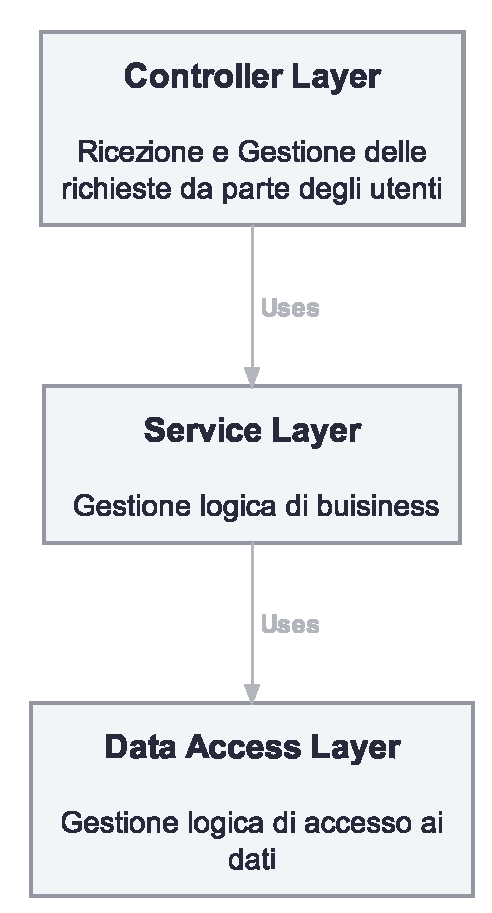
\includegraphics[width=0.35\textwidth]{three-tier.eps}
    \caption{Schema riassuntivo della architettura \textit{three-tier}}
    \label{fig:three-tier}
\end{figure}
\newpage

Questa architettura viene supportata grazie a dei componenti di base, offerti dal framework stesso, che possono
essere estesi dallo sviluppatore in base alle proprie esigenze.
Importante caratteristica di tutti questi componenti è che fanno largo uso della
\textit{Dependency Injection}\footnote{
    La \textit{Dependency Injection} è un meccanismo che permette di applicare
    l'inversione del controllo a un componente software. In generale permette a una classe di non dover configurare
    le proprie dipendenze in modo statico perché vengono configurate dall'esterno. Ciò offre grossi vantaggi in termini di riusabilità e rende la fase di test molto più semplice.}.

Pertanto l'utilizzo di Nest offre agli sviluppatori utili strumenti per velocizzare lo sviluppo di una web API prestando attenzione
alle performance e alla architettura software del prodotto da realizzare risultando un'ottima scelta per la realizzazione si servizi web.

\subsection{Testing}
\subsubsection{Jest}
Jest\cite{Jest} è un test runner JavaScript, sviluppato da Facebook, che fornisce un tool di strumenti per testare una applicazione basata su Node.js.

Permette una facile implementazione di unit test e integration test, con la possibilità di
sfruttare i \textit{mock objects} ("oggetti simulati"). Fornisce inoltre strumenti statistici per analizzare
la \textit{code coverage} ("copertura del codice").


